\documentclass[a4paper,12pt]{article}
\usepackage{amssymb}
\usepackage{amsfonts}
\usepackage{amsthm}
\usepackage{amsmath}
\usepackage[T1]{fontenc}
\usepackage[utf8]{inputenc}
\usepackage[british]{babel}
\usepackage{times}
\usepackage{anysize}
\usepackage{color}
\usepackage{listings}
\usepackage{graphicx}
\usepackage{enumerate}
\usepackage{multicol}
\usepackage{float}

\usepackage{lmodern}  % for bold teletype font
\usepackage{xcolor}   % for \textcolor
%\lstloadlanguages{matlab}
\lstset{
	basicstyle=\ttfamily,
	columns=fullflexible,
%	frame=single,
	breaklines=true,
	postbreak=\mbox{\textcolor{red}{$\hookrightarrow$}\space},
}

\begin{document}
\begin{titlepage}
\center
\vspace*{\fill}
\Huge{Modeling of Physical Systems}\\
\Large{Simulation of stress and strain distribution
using finite element method}\\
\vspace*{1.5cm}
Dominik Katszer\\
\large{23 June 2018}
\vspace*{1.5cm}
\vspace*{\fill}
\end{titlepage}
\section{Aim of laboratory}
The aim of this laboratory was to calculate, visualize and analyze stress and strain distribution for 2d models. What is more, this laboratory had to teach us how to use PDETool.

\section{Exercises}
During this laboratories we used pdetool, installed in Matlab. It is a program which allow us to draw the model, set
parameters and finally make a desired calculation. It also visualize result.
\subsection{Parameters}
\centerline{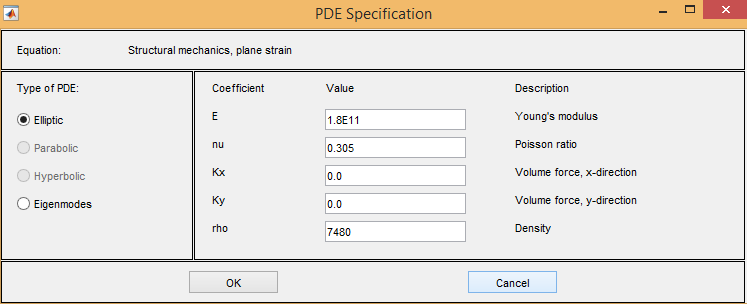
\includegraphics[scale=0.7]{stainless_Stell_properties}}
\centerline{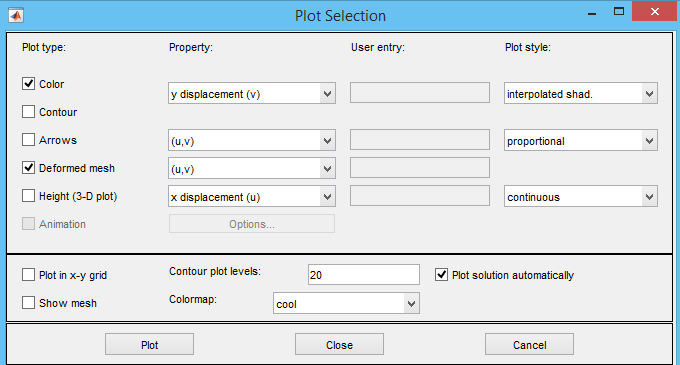
\includegraphics[scale=0.7]{plotParameters}}
\subsection{Mesh from laboratories}
\centerline{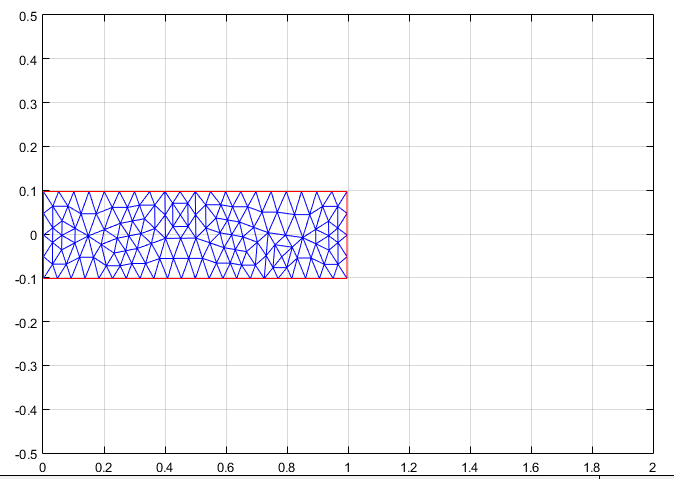
\includegraphics[scale=0.7]{meshFromLabs}}

Boundary conditions with applied forces: 
\begin{table}[H]
\centering
\begin{tabular}{|l|l|l|l|}
\hline 
Side  & Condition type & surface tractions & weights \\ \hline 
left  & Dirchlet & NA & h11, h22 = 1, h12, h21 = 0 \\ \hline 
top   & Dirchlet & NA & h11, h12, h21, h22 = 0 \\ \hline
right & Neumann  & g1 = 0, g2 = -1000 & NA \\ \hline
bottom   & Dirchlet & NA & h11, h12, h21, h22 = 0 \\ \hline

\end{tabular}
\caption{Boundary conditions settings}
\end{table}

\centerline{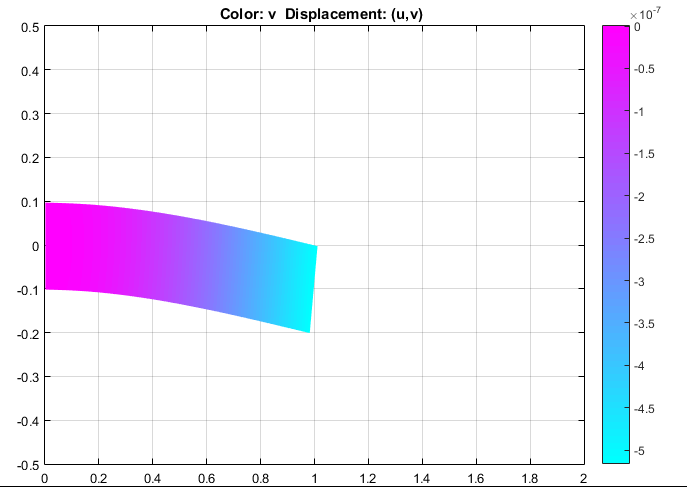
\includegraphics[scale=0.7]{resultFromLabs}}
\subsection{Theorethical value}
The value of deformation on the end of beam can be calculated using equation below
\begin{equation}
   h = \frac{F \cdot L^3}{3E \cdot J} \qquad
\end{equation}
For the rectangular cross section elastic modulus can be calculated from the equation:
\begin{equation}
\qquad J = \frac{g \cdot d^3}{12}
\end{equation}
Where:
\begin{itemize}
     \item $F = 1000 N$ - loading force
     \item $L = 1 m$ - beam length
     \item $E = 1.8 * 10^{11} Pa$ - Young's modulus
     \item $g = 1m$ - beam thickness
     \item $d = 0.2m$ - beam width
\end{itemize}
The theorethical result is :
\begin{lstlisting}
h =

  -2.7778e-06
\end{lstlisting}
Comparision between theorethical value and calculated by tool is presented in the tabular below.\\\\
\begin{tabular}{|l|l|l|l|}
\hline 
Method  & result \\ \hline 
Exported value from PDE tool& $-5.7840 \cdot 10^{-4}$  \\ \hline 
Theoretical value & $-2.7778 \cdot 10^{-6}$  \\ \hline
\end{tabular}\\\\
In my opinion the difference in this example is caused by not perfectly drawed beam in a tool. PDETool computes values more precisely because it can adjust applying math directly to the mesh.
\subsection{More complicated mesh}
\centerline{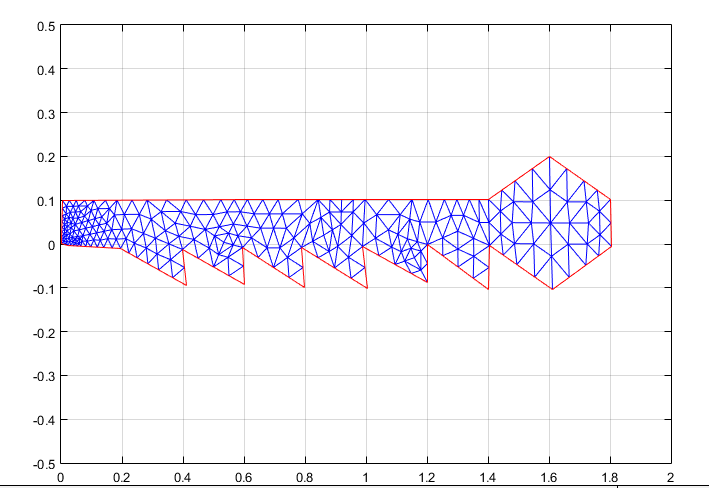
\includegraphics[scale=0.7]{myMesh}}
\centerline{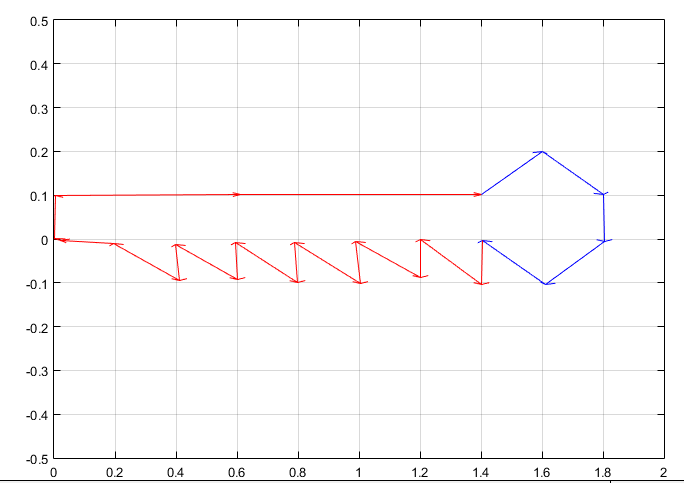
\includegraphics[scale=0.7]{myForces}}
\centerline{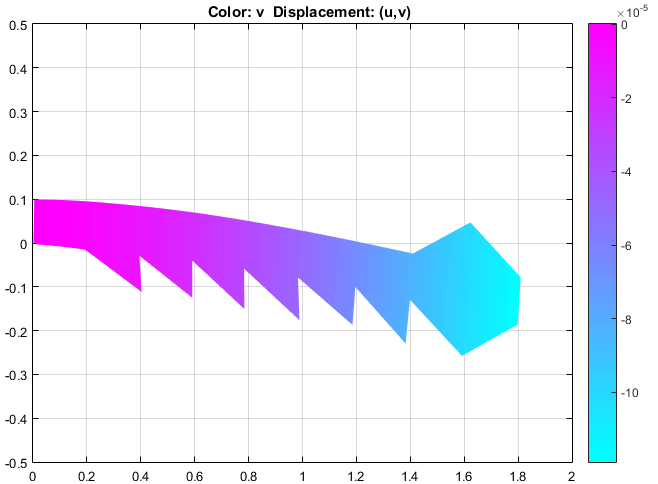
\includegraphics[scale=0.7]{myResult}}
\section{Conclusions}

This report covered stress and strain distribution. All needed calculations and visualisation were made in PDEtool which is quite intuitive. It allows to create complicated models and simulates different kinds of forces which affects on mesh. What is more, theoretical calculations were made for trivial model. It proves that despite the fact that results were not the same this tool is usable. The most important difference between simulation and theoretical calculations is visualisation as time needed for compute results. This two factors indicates that it is better to use tools for simulation with complex models.

\end{document}